\documentclass{report}
\usepackage[fontsize=13pt]{scrextend}
\usepackage{setspace}
\setstretch{1.25}
\usepackage[left=3.5cm,right=2cm,top=3.5cm,bottom=3cm]{geometry}
\usepackage{palatino} % Change font family
\usepackage[utf8]{vietnam} % For Vietnamese typing
\usepackage{graphicx} % For Image usage
\usepackage{tikz} % For drawing pictures
\usepackage{changepage} % For `adjustwidth` environment
\usepackage[hidelinks,unicode]{hyperref} % Make TOC clickable and hide the Red Border, using Unicode
\hypersetup{
    linkcolor=black % Set color of links as Black
}
\setcounter{tocdepth}{1} % Only show parts, chapters, and sections in TOC
\setlength\parindent{0pt} % No Indentation
\usepackage{amssymb} % For Mathematical symbols
\usepackage{amsmath} % For `align` environment

\begin{document}
\pagenumbering{gobble}
\begin{titlepage}
    \centering
    \vspace{0.25cm}
    {\large Trường Đại học Bách Khoa Hà Nội\par}
    \vspace{0.25cm}
    {\normalsize Viện Toán ứng dụng và Tin học\par}
    \vspace{0.75cm}
    {
\includegraphics[width=69px]{anh/hust-logo.png}\par}
    \vspace{1.25cm}
    {\Large\textbf{BÁO CÁO THỰC TẬP KĨ THUẬT}\par}
    \vspace{1.5cm}
    {\large Cấp phát nội dung số trên chuỗi khối\par}
    \vspace{0.25cm}
    {\large sử dụng hệ thống tập tin liên hành tinh\par}
    \vspace{1.5cm}
    \begin{flushleft}
        \hspace{3cm}
        {\normalsize\textit{Doanh nghiệp:}\par}
        \vspace{0.125cm}
        \hspace{5cm}
        {\normalsize Division 6 \textit{- Công ty cổ phần Rikkeisoft}\par}
        \vspace{0.125cm}
        \hspace{3cm}
        {\normalsize\textit{Thực hiện:}\par}
        \vspace{0.125cm}
        \hspace{5cm}
        {\normalsize Đỗ Minh Tuấn \textit{- 20185419}\par}
    \end{flushleft}
    \vspace{3cm}
    {\normalsize Hà Nội, 2022\par}
    \vspace{0.5cm}
\end{titlepage}
\newpage
\thispagestyle{empty} % Not numbered this page
\section*{
    \centering
    Nhận xét của giảng viên hướng dẫn
    \vspace{1.25cm}
}

\subsection*{Mục đích và nội dung của Đồ án}
\begin{tikzpicture}
    \draw[draw=black] (0,0) rectangle ++(15,2.5);
\end{tikzpicture}

\subsection*{Kết quả đạt được}
\begin{tikzpicture}
    \draw[draw=black] (0,0) rectangle ++(15,2.5);
\end{tikzpicture}

\subsection*{Ý thức làm việc của sinh viên thực hiện}
\begin{tikzpicture}
    \draw[draw=black] (0,0) rectangle ++(15,2.5);
\end{tikzpicture}

\begin{adjustwidth}{200pt}{0pt}
    \vspace{1cm}
    {\textit{Hà Nội, ngày ... tháng ... năm ...}\par}
    \vspace{0.25cm}
    {\textbf{Giảng viên hướng dẫn}\par}
    \vspace{0.25cm}
    \hspace{0.75cm}{\textit{(Ký và ghi rõ họ tên)}\par}
\end{adjustwidth}
% \section*{
    \centering
    Tóm tắt nội dung của Đồ án
    \vspace{1.25cm}
}

\subsection*{Mục đích của Đồ án}

Đồ án \textit{Ứng dụng Chuỗi khối trong quản lý văn bằng giáo dục} cung cấp những cái nhìn tổng quan về vấn đề xác thực "bằng thật - bằng giả" giữa nhà tuyển dụng và ứng viên; thực trạng và tính minh bạch của các hệ thống tra cứu hiện có; đồng thời đưa ra giải pháp sử dụng công nghệ \textit{chuỗi khối} cho quá trình cấp phát và tra cứu văn bằng.

\subsection*{Các công nghệ đã sử dụng}

Ngoài cơ sở lý thuyết về \textit{chuỗi khối} cùng với \textit{mật mã hoá bất đối xứng}, phần triển khai của đồ án có sử dụng các công nghệ sau:
\begin{itemize}
    \item \textit{Mạng Ethereum}: Nơi triển khai các \textit{hợp đồng thông minh} - chương trình thực thi trên mạng phân tán, nơi dữ liệu được thay đổi dựa trên tính đồng thuận của toàn mạng.
    \item \textit{Giao thức IPFS}: Một giao thức cho phép lưu trữ và phân phối tập tin trên một mạng ngang hàng phân tán một cách bảo mật và tiết kiệm bộ nhớ.
\end{itemize}

Bên cạnh đó, \textit{hệ thống cấp phát văn bằng} được xây dựng để dễ dàng thao tác với \textit{ví MetaMask} - một chương trình lưu trữ \textit{khoá bí mật} cung cấp các tính năng để tương tác với các \textit{mạng chuỗi khối} một cách thân thiện và an toàn.


\section*{
    \centering
    Lời cảm ơn
    \vspace{1.25cm}
}

Khoảng thời gian được làm việc trong môi trường doanh nghiệp đem lại cho em rất nhiều kinh nghiệm, cũng như những kiến thức chuyên ngành quý giá. Em xin gửi lời cảm ơn tới toàn thể anh, chị tại \textit{Công ty cổ phần Rikkeisoft}\footnote{\href{https://rikkeisoft.com/}{https://rikkeisoft.com/}}, đặc biệt là anh \href{mailto:luattv@rikkeisoft.com}{\textit{Trần Văn Luật}} (\textit{Sub-Leader} của \textit{Division 6}), mọi người đã giúp đỡ em rất nhiều trong quá trình học tập tại đây. Em xin cảm ơn mọi người.\\

Tuy một học kỳ là ngắn ngủi, nhưng với định hướng rõ ràng, quả thực, nó mang lại cho em quá là nhiều kiến thức, đưa em đến những chân trời mới về công nghệ. Sau mỗi thành tựu mà ai đó đạt được, sẽ thật thiếu sót khi không nhìn vào sự nỗ lực của chính họ. Bản thân em cũng đã dành ra khá nhiều công sức tìm hiểu, thử nghiệm, triển khai, và mang đến kết quả phù hợp nhất cho đề tài mà mình đã chọn. Em tự tin với chất lượng của bài báo cáo này.\\
\pagebreak
\setcounter{page}{0} % Set the page counter to 0 in this page
\thispagestyle{empty} % Not numbered this page
\tableofcontents
\pagenumbering{arabic}
% --- Contents ---
\setcounter{page}{1} % Set the page counter to 0 in this page
\chapter{Tổng quan về bài toán cấp phát nội dung số}

Đã từ lâu, các doanh nghiệp cũng như các cá nhân bắt đầu lựa chọn các nền tảng đám mây cho mục đích lưu trữ dữ liệu. Những nhà cung cấp dịch vụ phổ biến hiện nay có thể kể đến như Google với \textit{Google Drive}, Microsoft với \textit{OneDrive}, DropBox, vân vân. Các dịch vụ này tương đối quen thuộc với hầu hết mọi người, hỗ trợ lên tới \textit{15GiB} dữ liệu cho người dùng không trả phí (miễn phí).\\

Do phổ biến như vậy, các doanh nghiệp dần triển khai làm việc trên các dịch vụ này. Dễ dàng nhận thấy rằng, những chứng nhận (như chứng chỉ, văn bằng, huy chương của các cuộc thi, vân vân) đã có thể lưu trữ và phân phối trên nền tảng số. Nhiều doanh nghiệp thậm chí đã chấm dứt cấp phát dưới dạng vật lý (giấy tờ, các vật liệu giả kim hoặc kim loại, vân vân) để giảm thiểu chi phí sản xuất. Cũng có nhiều doanh nghiệp tự xây dựng hệ thống lưu trữ đám mây cho riêng mình để thuận tiện quản lý.\\

Tuy nhiên, việc phụ thuộc vào một nhà cung cấp dịch vụ cũng đem đến rủi ro. Với sự gia tăng ngày càng nhiều của các vụ tấn công nhằm vào các nhà cung cấp dịch vụ đám mây, "khách hàng" chưa hoàn toàn yên tâm trong việc lưu trữ dữ liệu. Không ít các cuộc tấn công như vậy khiến dữ liệu bị sai lệch, không thể khôi phục lại được, hoặc có thể khôi phục lại nhưng dữ liệu không được như ban đầu. Rất nhiều giải pháp khác được thảo luận nhằm đảm bảo cho việc lưu trữ nội dung trên nền tảng số trở lên an toàn hơn.\\
\chapter{Chuỗi khối và mạng Ethereum}

\section{Tổng quan về chuỗi khối}

Một chuỗi khối là một sổ cái điện tử \textit{phân tán}\footnote{Distributed}, \textit{phi tập trung}\footnote{Decentralized}, bao gồm các bản ghi được gọi là \textit{khối} (block) thường được dùng để ghi lại các \textit{giao dịch} (transaction) qua các máy tính. Nói một cách dễ hiểu, chuỗi khối là một cơ chế cơ sở dữ liệu tiên tiến cho phép chia sẻ thông tin minh bạch trong một mạng lưới. Cơ sở dữ liệu chuỗi khối lưu trữ dữ liệu trong các khối được liên kết với nhau trong một chuỗi. Dữ liệu có sự nhất quán theo trình tự thời gian vì bạn không thể xóa hoặc sửa đổi chuỗi mà không có sự đồng thuận từ mạng lưới. Do đó, chuỗi khối được coi như một sổ cái không thể chỉnh sửa hay biến đổi để theo dõi các thông tin theo thời gian.

\section{Mạng Ethereum}

\subsection{Lịch sử}

Ethereum là một nền tảng mã nguồn mở dựa trên chuỗi khối, hỗ trợ \textit{Hợp đồng thông minh}\footnote{Smart contract}. Ethereum khá nổi với \textit{đồng tiền mã hoá}\footnote{Cryptocurrency} của nó với tên gọi là \textit{Ether} (ký hiệu: ETH). Dựa vào sự phân tán của công nghệ chuỗi khối, Ethereum khá an toàn, và cũng nhờ bảo mật cao nên giá trị của đồng tiền ETH tích luỹ ngày càng lớn trên thị trường tiện điện tử.\\

Bắt đầu ý tưởng từ năm 2013 bởi lập trình viên \href{https://en.wikipedia.org/wiki/Vitalik_Buterin}{\textit{Vitalik Buterin}} và một số cộng sự, công việc phát triển Ethereum được vận hành và kêu gọi vốn từ cộng đồng vào năm sau đó. Mạng Ethereum chính thức "lên sóng" vào ngày 30 tháng 7 năm 2015.\\

\subsection{Hợp đồng thông minh}

Nền tảng Ethereum còn hỗ trợ mạng lưới các \textit{ứng dụng phi tập trung}\footnote{Decentralized applications (DApps)}. Mạng này vận hành xoay quanh các hợp đồng thông minh. Phần lớn các ứng dụng sử dụng hợp đồng thông minh để liên kết với công nghệ chuỗi khối. Có thể nói, hợp đồng thông minh chính là nhân tố trung tâm của nền tảng Ethereum.\\

Hợp đồng thông minh là \textit{hợp đồng tự thực thi}\footnote{Self-executed contract} với các điều khoản được viết bởi các dòng lệnh hay các đoạn mã lập trình. Các đoạn mã này tồn tại khắp các nút trong mạng chuỗi khối, điều hành sự thực thi các giao dịch, và không thể thay đổi. Hợp đồng thông minh mang đến các giao dịch đáng tin cậy, sự đồng ý với các điều khoản trong hợp đồng tới các bên "ẩn danh" mà không cần qua một bên trung gian hay một cơ chế thực thi bên ngoài.\\

Trên Ethereum, các đoạn mã của hợp đồng thông minh được viết bằng ngôn ngữ lập trình \textit{Solidity} hoặc \textit{Vyper}. Solidity là ngôn ngữ lập trình hướng đối tượng bậc cao dựa theo \textit{C++}, \textit{JavaScript}, \textit{Python}, và được thiết kế để tích hợp được với \textit{Máy ảo Ethereum}\footnote{Ethereum Virtual Machine - EVM} (EVM). Vyper là ngôn ngữ đang trong quá trình thử nghiệm.\\

\subsection{Chi phí giao dịch}

\textit{Gas} là đơn vị thể hiện cho khối lượng tính toán để thực hiện một hành động nào đó trên mạng Ethereum. Do mỗi giao dịch trên mạng Ethereum đều cần tài nguyên tính toán để được thực thi, vì thế mà nó phát sinh ra \textit{chi phí giao dịch}. Khi đó, \textit{gas} thể hiện chi phí để thực hiện giao dịch thành công trên mạng.\\

\begin{figure}[ht]
    \centering
    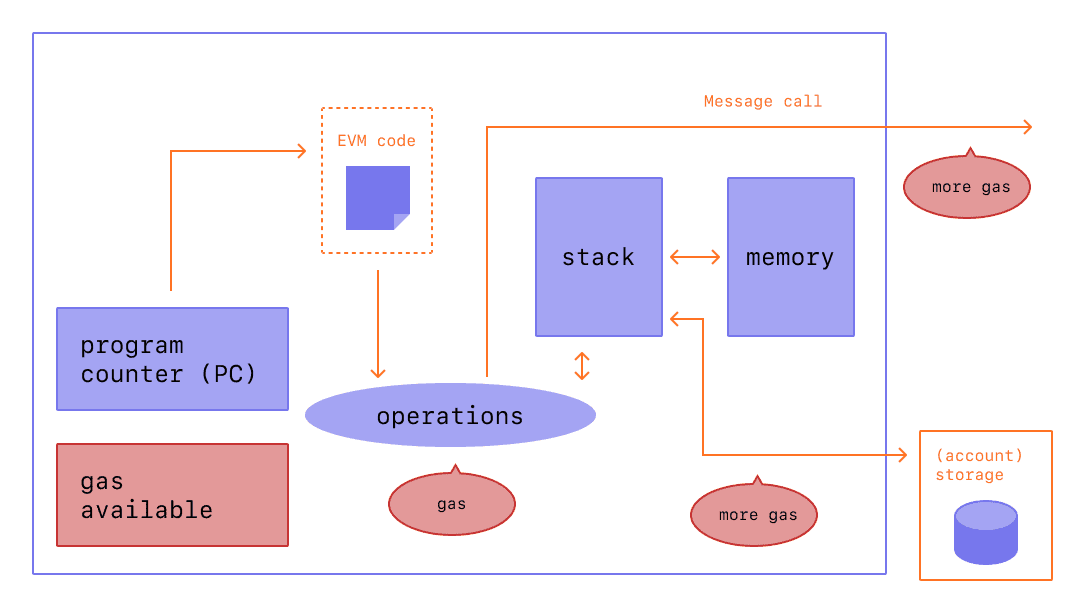
\includegraphics[width=400px]{images/gas.png}
\end{figure}

\textit{Gas} được trả bằng đồng \textit{ether} (ETH). \textit{Giá gas}\footnote{Gas price} có đơn vị là \textit{gwei}, mỗi \textit{gwei} tương ứng với một phần một tỷ của một \textit{ether}: $1$ \textit{gwei} $=10^{-9}$ \textit{ether}. Vì vậy, thay vì nói chi phí giao dịch là $0,000000001$ \textit{ether}, ta có thể nói giao dịch đó tiêu tốn $1$ \textit{gwei}. Ngoài ra, $1$ \textit{gwei} chính là một tỷ \textit{wei}; \textit{wei} (được đặt tên theo \textit{Wei Dai} - nhà khoa học máy tính nổi tiếng đưa ra lý thuyết về thanh toán bằng tiền mã hoá) là đơn vị nhỏ nhất trên Ethereum.\\


\chapter{Hệ thống tập tin phân tán IPFS}

\section{Tổng quan về IPFS}

IPFS là viết tắt của từ Interplanetary File System, một hệ thống tập tin phân tán ngang hàng kết nối tất cả các thiết bị máy tính với nhau. Cụ thể hơn, nó sẽ phân phối dữ liệu được lưu trữ theo hình thức P2P, hay còn gọi là mạng ngang hàng (mạng đồng đẳng).\\

Trong đó, các hoạt động của IPFS chủ yếu dựa vào khả năng tính toán băng thông của tất cả các máy tham gia chứ không tập trung vào một phần nhỏ các máy chủ trung tâm như giao thức HTTP. Nói cách khác, IPFS là mạng lưới chuyển phát nội dung hoàn toàn phi tập trung cho phép quản lý và lưu trữ dữ liệu một cách linh hoạt. Mỗi máy tính tham gia trong mạng lưới đảm nhận nhiệm vụ download và upload dữ liệu mà không cần sự can thiệp của máy chủ trung tâm.\\



\section{Cơ chế hoạt động}

\section{Điểm độc đáo của IPFS}

Nếu được triển khai đúng, IPFS mang lại tiềm năng lớn nhờ cải thiện được tốc độ truyền tải dữ liệu, tránh sự phụ thuộc vào các máy chủ và tiết kiệm chi phí.

\subsection{Tránh sự phụ thuộc vào máy chủ}

Trong các mô hình Máy khách - Máy chủ như HTTP, khi các máy chủ đang gặp phải sự cố thì chúng sẽ không thể hồi đáp thông tin cho người dùng. Đây cũng là vấn đề lớn nhất mà giao thức HTTP gặp phải khi nó phụ thuộc vào một máy chủ tập trung, điều mà nó không thể cải thiện cũng như khắc phục.\\

Với IPFS, nó hoàn toàn bỏ qua khái niệm máy chủ, mà chỉ quan tâm tới nội dung tìm kiếm. Điều này không chỉ giúp chúng ta rút ngắn con đường tới thông tin, mà lại không lo gặp phải các máy chủ kém chất lượng, kém tin cậy.

\subsection{Mô hình phi tập trung}

Với một mô hình tập trung, số lượng lớn dữ liệu được tập trung trong tay một số tên tuổi lớn trong lĩnh vực như Facebook, Amazon, Google,... Điều này vô tình khiến chúng trở thành tâm điểm cho các tin tặc tấn công. Trong lịch sử, không ít lần chúng ta chứng kiến những vụ rò rỉ thông tin liên quan đến những tên tuổi lớn.\\

Với mô hình phi tập trung của IPFS, các vấn đề này hoàn toàn được khắc phục và không còn chế độ quản lý phân cấp. Các dữ liệu được lưu trữ phân tán và không có một máy chủ tập trung để tấn công, càng nhiều người tham gia vào IPFS thì mạng sẽ càng bảo mật và khó có thể thao túng hơn.

\subsection{Giảm bớt chi phí}

Ưu điểm tiếp theo của mô hình IPFS đó là giảm bớt chi phí đối với cả người cung cấp nội dung và người dùng thông thường. IFPS sẽ cho phép đoạn video trên được tải hoàn toàn về mạng nội bộ IFPS dù bạn là ai và đang ở đâu. Do đó loại bỏ sự cần thiết của hàng loạt trạm kết nối và máy chủ Internet, giúp chi phí tổng thể giảm một cách rõ rệt.


\section{Bảo mật và quyền riêng tư}
\chapter{Quản lý văn bằng giáo dục trên mạng Ethereum}

\section{Đề xuất giải pháp}

Giải pháp phổ biến hiện nay là xây dựng cơ sở dữ liệu chung về văn bằng giữa các cơ sở giáo dục. Nhà tuyển dụng có thể dễ dàng tra cứu thông tin văn bằng khi truy cập vào hệ thống sử dụng cơ sở dữ liệu này. Tuy nhiên, vấn đề hiện hữu là sử dụng cơ sở dữ liệu chung truyền thống tiềm ẩn rất nhiều rủi ro về dữ liệu. Việc nhiều bên truy cập và chỉnh sửa dữ liệu (các cơ sở giáo dục có quyền như nhau đối với cơ sở dữ liệu này) có thể phát sinh mất mát và ảnh hưởng đến dữ liệu của các bên khác. Ngoài ra, nếu giao quyền cập nhật dữ liệu cho một hoặc một số lượng hạn chế các bên tham gia, quy trình rà soát và sửa sai có thể kéo dài và các yêu cầu thay đổi dữ liệu được gửi từ các bên không có quyền cập nhật sẽ không được xử lý kịp thời.\\

Không phải nói quá, chuỗi khối giải quyết quá tốt các bài toán về cơ sở dữ liệu chung, đặc biệt là khi tính minh bạch của dữ liệu được ưu tiên. Đặc biệt, tương tác với chuỗi khối ngày càng trở nên đơn giản với \textit{DApp} - các ứng dụng phi tập trung với giao diện thân thiện, dễ dùng, đồng thời tốc độ truy xuất thông tin chấp nhận được, việc ứng dụng chuỗi khối càng được ưa chuộng. Việc lưu trữ thông tin văn bằng giáo dục trên chuỗi khối đảm bảo được dữ liệu không thể bị chỉnh sửa, mọi người đều dễ dàng truy cập. Nhiệm vụ cấp phát văn bằng được đưa về phía từng cơ sở giáo dục, lưu trữ trên mạng chuỗi khối chung, không thể chỉnh sửa. Đó là ưu điểm khi việc quản lý văn bằng sẽ không quá tập trung vào một số bên nhất định, nhưng cũng là thách thức cho các cơ sở giáo dục trong vấn đề xây dựng hệ thống tích hợp với mạng chuỗi khối một cách hợp lý và tốn không quá nhiều chi phí.
\newpage
\section{Xây dựng hệ thống}

Với yêu cầu của bài toán, ta cần xây dựng hệ thống cấp phát cho các doanh nghiệp, và hệ thống tra cứu thông tin nội dung cho người có nhu cầu tra cứu.\\

\begin{figure}[ht]
    \centering
    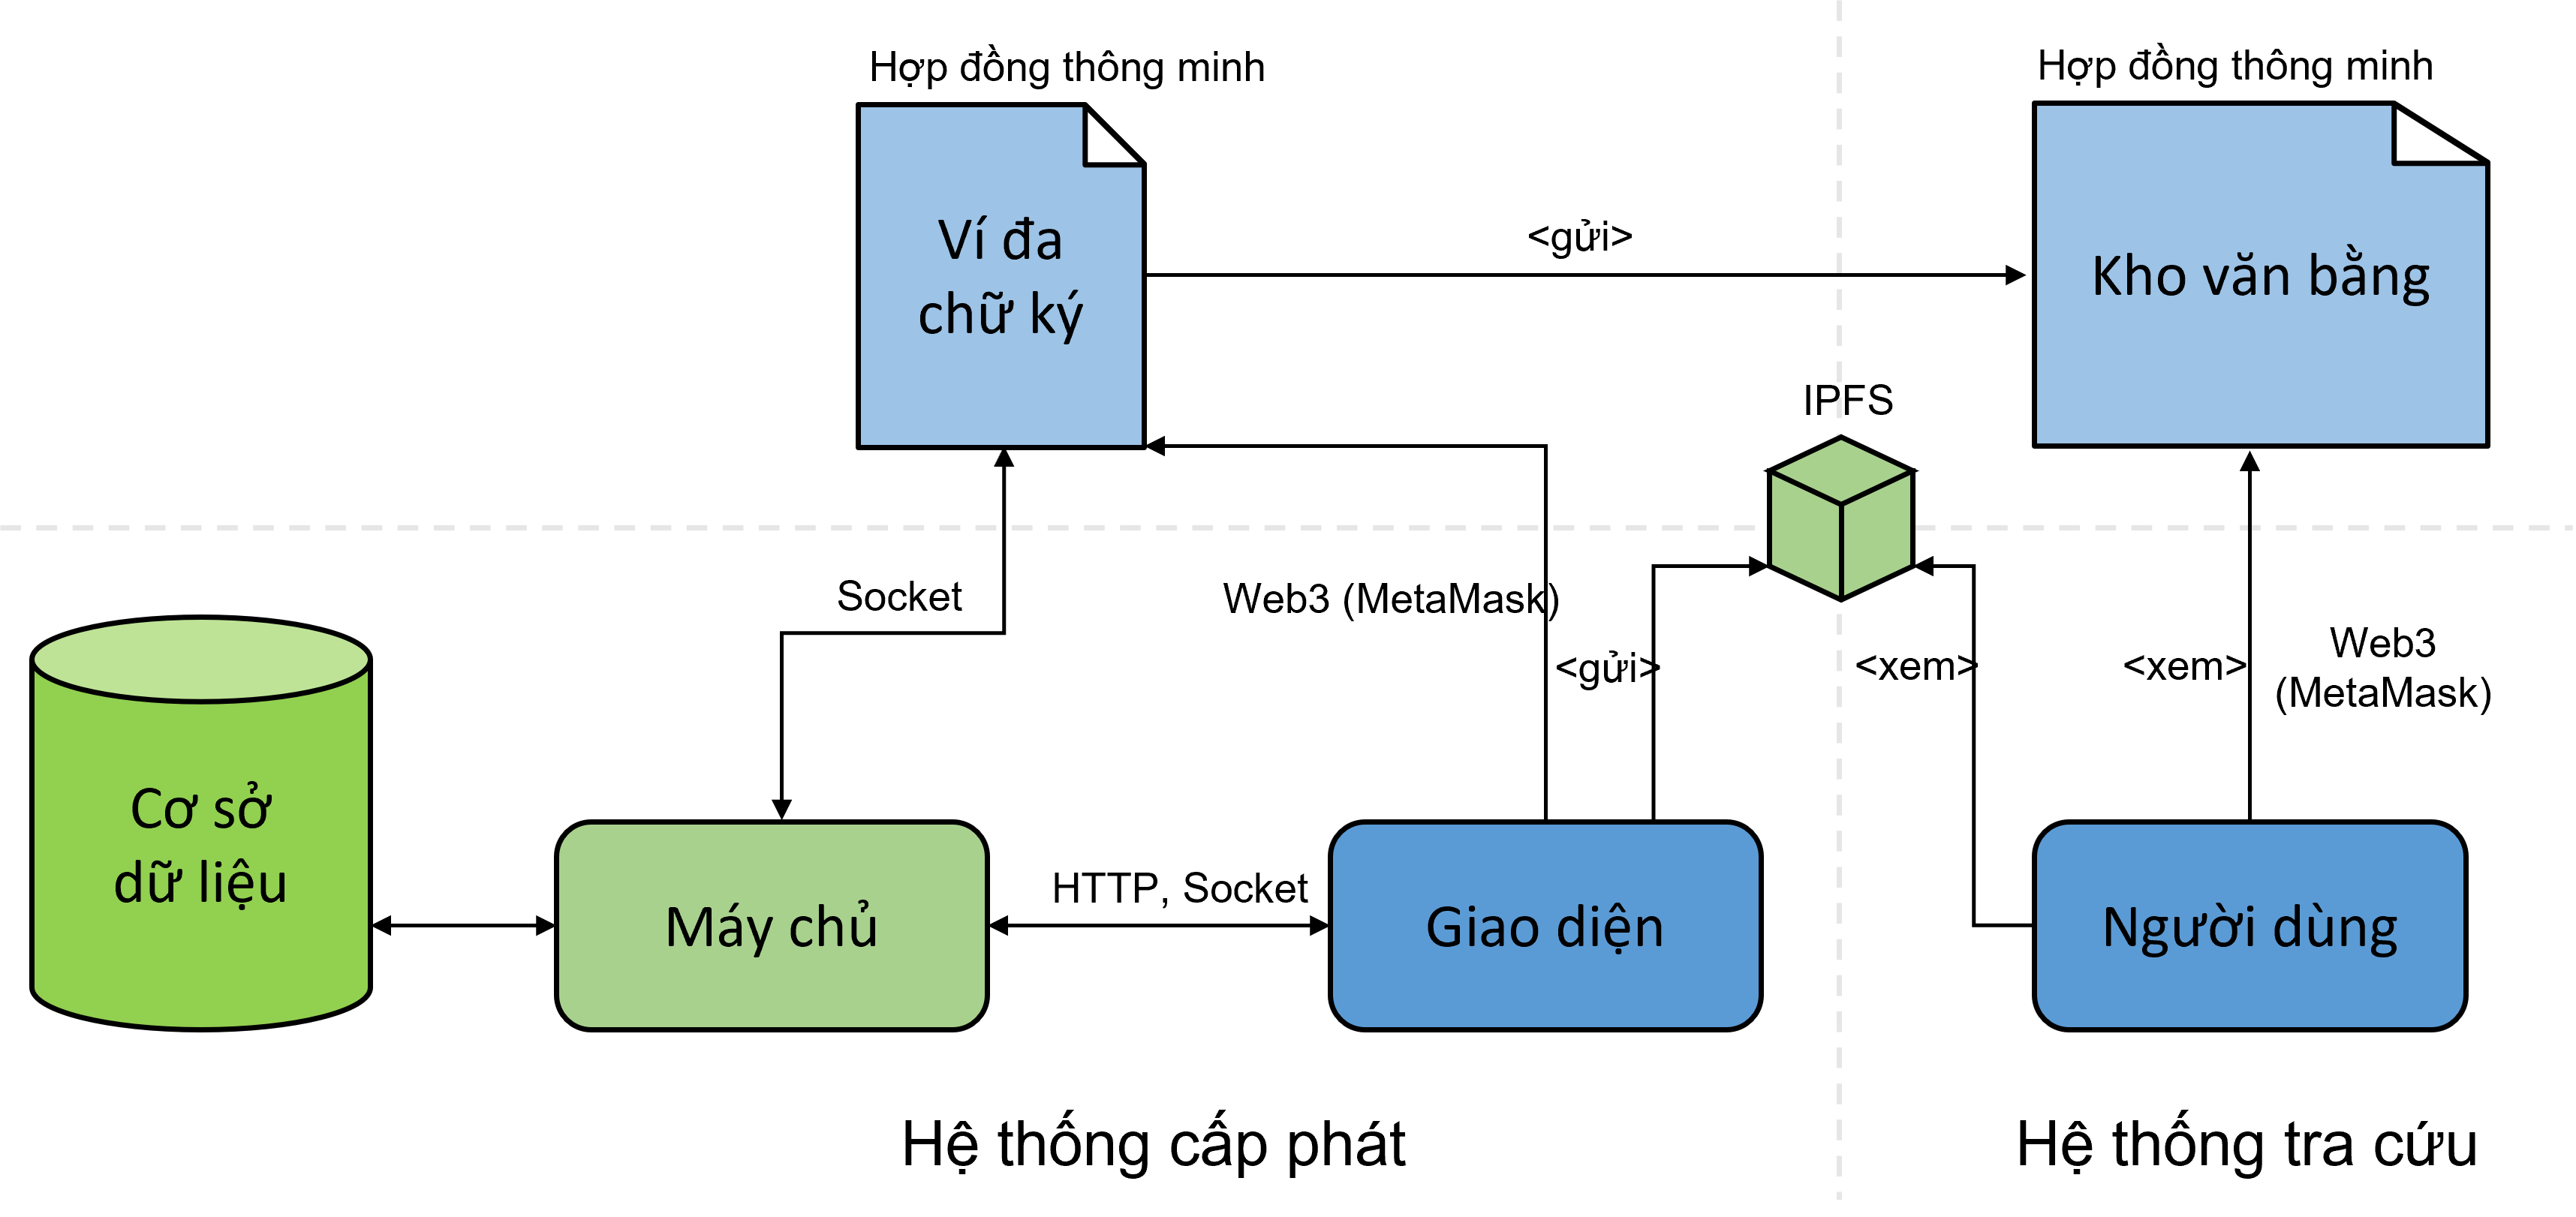
\includegraphics[width=400px]{anh/giai-phap/tong-quan-he-thong.png}
    \caption{Sơ đồ tổng quan các hệ thống và mạng chuỗi khối}
    \label{images/system-overview}
\end{figure}

Những hệ thống này sẽ tương tác với các hợp đồng thông minh trên mạng chuỗi khối, bao gồm \textit{Kho nội dung} và \textit{Ví đa chữ ký}. Trong bài báo cáo này, em xin phép tập trung trình bày về phần thiết kế các hợp đồng thông minh được triển khai cùng hệ thống.


\subsection{Kho nội dung}
\textit{Kho nội dung} là một hợp đồng thông minh nắm giữ thông tin các nội dung được lưu trữ trên mạng chuỗi khối. Thông tin được tổ chức theo cấu trúc dạng cây, mỗi mã số nội dung trên mạng chuỗi khối sẽ tương ứng với các thông tin liên quan đến nội dung đã được cấp phát.\\

Để lưu trữ nội dung trên mạng chuỗi khối, các cơ sở cấp phát cần sử dụng một địa chỉ ví để tương tác với hợp đồng thông minh được triển khai trên mạng đó. Mỗi cơ sở phát hành nội dung sẽ có một địa chỉ ví xác định, là chữ ký đại diện cho cơ sở cấp phát nội dung đó.\\

\begin{figure}[!ht]
    \centering
    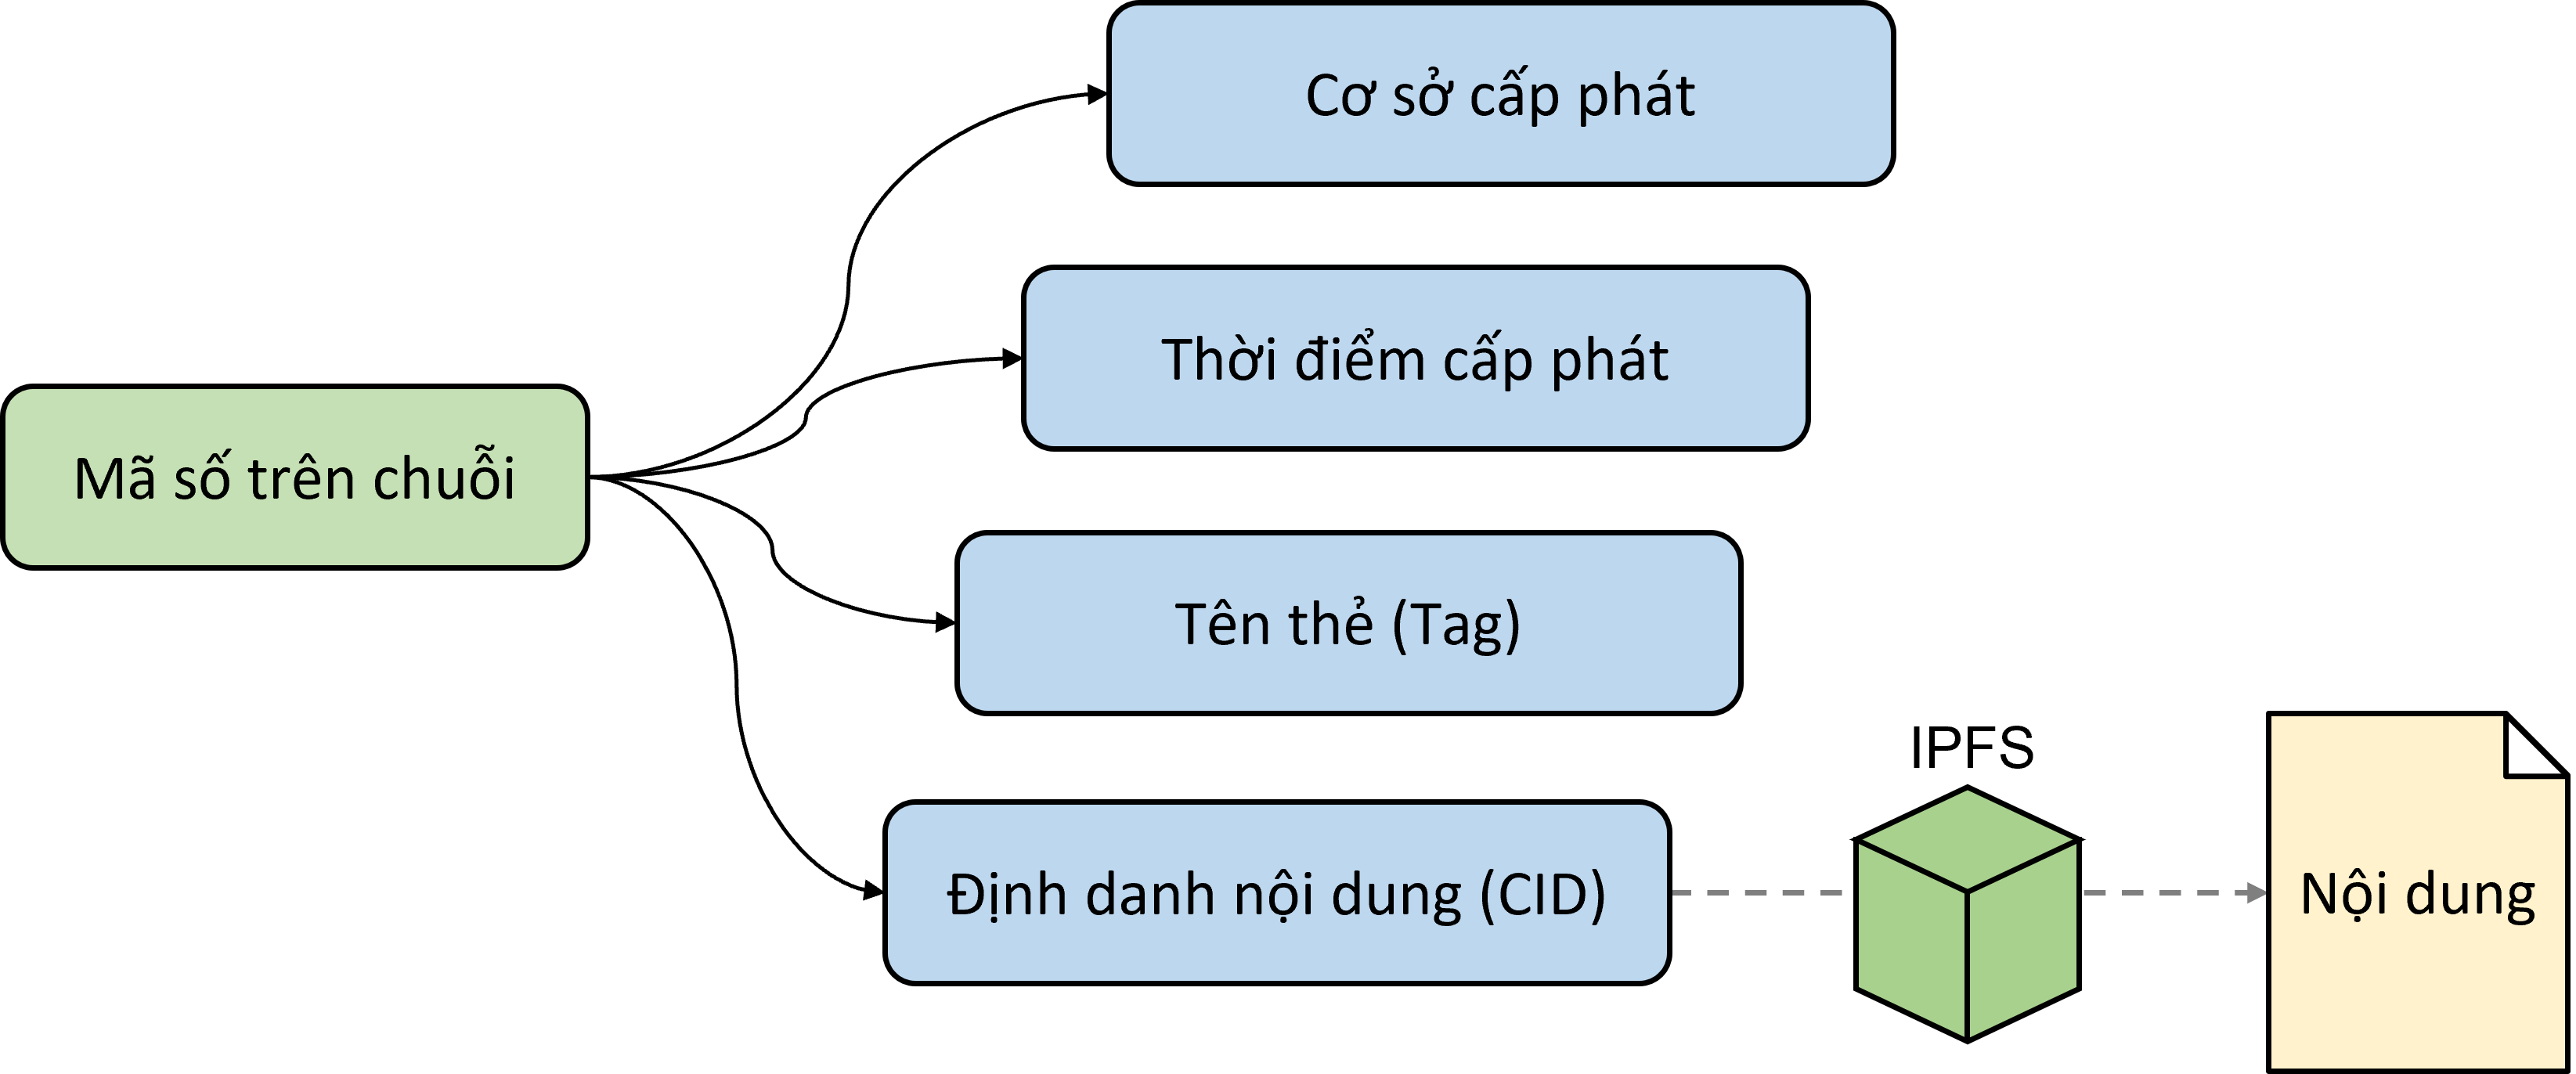
\includegraphics[width=400px]{anh/giai-phap/cau-truc-du-lieu.png}
    \caption{Cấu trúc lưu trữ thông tin trong \textit{kho nội dung}}
\end{figure}

\textit{Kho nội dung} cung cấp một số chức năng liên quan đến lưu thông tin, tra cứu thông tin nội dung. Cụ thể, ba chức năng hiện có ở đây là:
\begin{itemize}
    \item Lưu thông tin nội dung
    \item Xem thông tin nội dung
    \item Khoá nội dung
\end{itemize}

Đối với việc \textit{lưu thông tin}, địa chỉ ví của cơ sở (hay người) gửi yêu cầu lưu thông tin nội dung sẽ được lấy làm \textit{Cơ sở cấp phát}, và thông tin đi kèm sẽ được sử dụng làm \textit{Tên thẻ} cho nội dung. Như vậy, sẽ không có tình huống một cơ sở cấp phát phát hành nội dung với địa chỉ của cơ sở khác, trường hợp nhầm lẫn do vô ý hoặc có chủ đích không thể xảy ra.\\

Để \textit{xem thông tin}, người tra cứu chỉ cần cung cấp mã số nội dung đã được cấp phát. Những thông tin được hợp đồng thông minh trả về bao gồm cả định danh nội dung trên mạng IPFS, hệ thống tra cứu sẽ tự động lấy nội dung nội dung (bao gồm cả phụ lục nội dung) dựa trên định danh này.\\

Đối với trường hợp nội dung đã được cấp phát nhưng thông tin bị sai hoặc không phù hợp, phía cơ sở cấp phát nội dung có thể lựa chọn \textit{khoá nội dung} lại. Người tra cứu không thể \textit{xem thông tin} đối với những nội dung đã bị khoá.

\subsection{Ví đa chữ ký}
\textit{Ví đa chữ ký} là một hợp đồng thông minh với mục đích tăng tính bảo mật cho quá trình tương tác thay đổi thông tin nội dung trên chuỗi khối.\\

Với việc "đẩy" thông tin nội dung lên mạng chuỗi khối một cách thông thường, mỗi cơ sở cấp phát sử dụng địa chỉ ví của một cá nhân đại diện để tương tác, hoặc lựa chọn một địa chỉ ví và sử dụng chung cho cá nhân trong cơ sở. Điều này đảm bảo mỗi cơ sở cấp phát chỉ có một địa chỉ duy nhất. Tuy nhiên, khi nhiều cá nhân cùng dùng một địa chỉ ví, khả năng mất cắp tài sản liên kết với địa chỉ này càng lớn, đặc biệt khi nó còn được sử dụng trong các giao dịch khác có giá trị về tài chính (như địa chỉ sở hữu tiền mã hoá với giá trị cao trên các \textit{sàn giao dịch}\footnote{Exchange}, hay liên kết với các \textit{DApp} khác). Do đó, một cơ chế giúp giảm thiểu khả năng nhiều người cùng sở hữu một địa chỉ ví và có thể sử dụng địa chỉ ví để xác thực thông tin cơ sở cấp phát nội dung là vô cùng cần thiết. \textit{Ví đa chữ ký} ra đời để giải quyết vấn đề này.\\

Không giống với các \textit{hệ thống xác thực đa chữ ký}\footnote{Multi-signature authentication system} khi ít nhiều phụ thuộc vào các cơ chế xác thực phức tạp, \textit{ví đa chữ ký} sử dụng các tính năng, lợi thế của hợp đồng thông minh và mạng chuỗi khối. Ở \textit{ví đa chữ ký}, mỗi hành động cần thực thi (ở đây là việc cấp phát nội dung) yêu cầu một số lượng nhất định sự đồng ý từ cá nhân. Địa chỉ ví của các cá nhân này đã được thêm vào danh sách "thành viên" ngay từ khi hợp đồng thông minh này được triển khai, và họ được coi như các "cổ đông" của "doanh nghiệp" cấp phát nội dung khi có "tiếng nói" trong các "hoạt động" ở đây. Mỗi cơ sở cấp phát nội dung sử dụng một \textit{ví đa chữ ký} duy nhất, và địa chỉ của hợp đồng thông minh này đại diện cho địa chỉ ví của cả cơ sở đó. Các nội dung cần được đẩy lên \textit{kho nội dung} sẽ được một cá nhân trong cơ sở gửi lên "ví" này. Các thành viên khác trong cơ sở có thể xem thông tin các nội dung được gửi lên, và đưa ra biểu quyết "đồng ý" hay "không đồng ý" trên hợp đồng thông minh. Khi số lượng sự đồng ý đạt ngưỡng nhất định (được thiết lập từ đầu), các nội dung đó được đẩy lên "kho", và thông tin được lưu trữ trên mạng chuỗi khối.\\

\begin{figure}[!ht]
    \centering
    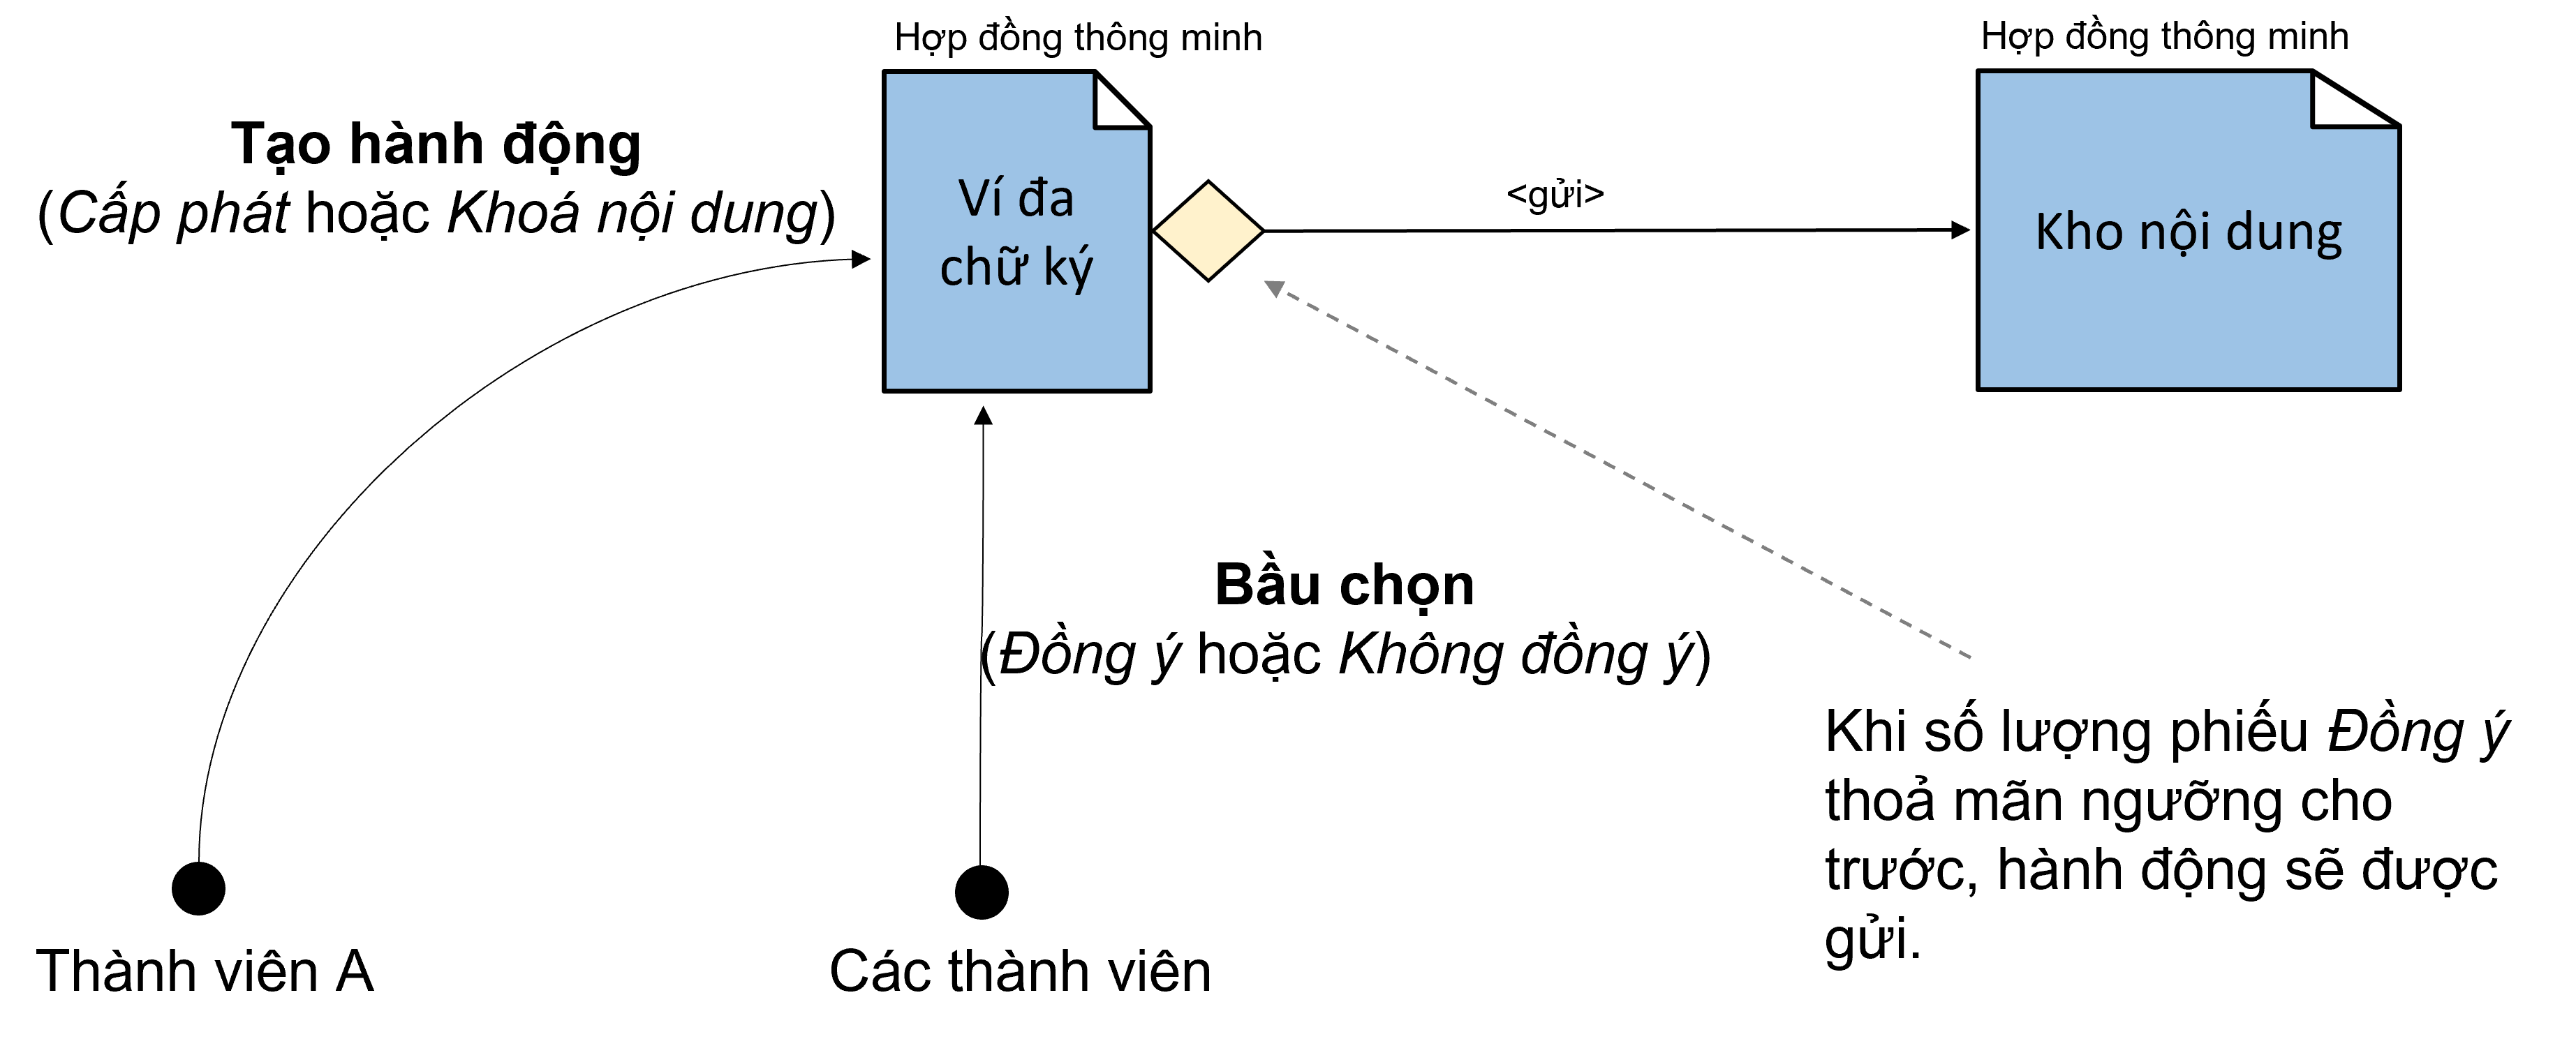
\includegraphics[width=400px]{anh/giai-phap/co-che-bau-chon.png}
    \caption{Cơ chế bầu chọn trong hệ thống}
\end{figure}


\newpage
\section{Kết quả triển khai và đánh giá}

\subsection*{Triển khai}

Giao diện \textit{hệ thống quản lý} được xây dựng với thư viện \href{https://reactjs.org}{\textit{React}} (được phát triển bởi đội ngũ \textit{Facebook} với sự đóng góp của cộng đồng) sử dụng ngôn ngữ lập trình \href{https://www.typescriptlang.org/}{\textit{TypeScript}}. Đồng thời, người dùng cần đồng ý kết nối ví mã hoá \textit{MetaMask} với hệ thống để sử dụng các tính năng tương tác với hợp đồng thông minh. Phía máy chủ, \href{https://nodejs.org}{\textit{Node.js}} được lựa chọn, ta sử dụng \href{https://expressjs.com/}{\textit{Express}} để tạo các \textit{API}\footnote{Application Programming Interface}. Thông tin cần thiết được lấy từ cơ sở dữ liệu, và việc trao đổi giữa máy chủ và giao diện được thực hiện qua kết nối \textit{HTTP} và \textit{Web Socket}, các cập nhật từ một người sẽ được thông báo ngay lập tức tới các cá nhân khác trong cùng cơ sở cấp phát văn bằng.\\

\textit{Hệ thống tra cứu} sử dụng cấu trúc \textit{trang tĩnh}\footnote{Static web}, triển khai trên \textit{GitHub Pages} với mã nguồn công khai, cung cấp cho người dùng một công cụ tra cứu thông tin văn bằng nhanh chóng, đáng tin cậy. Các doanh nghiệp có thể lấy danh sách \textit{địa chỉ ví} của các cơ sở giáo dục tại trang thông tin (website) của cơ sở giáo dục đó, hoặc lấy từ một cơ quan có độ tin cậy lớn (như \textit{Bộ Giáo dục và Đào tạo} chẳng hạn). Thông tin số hiệu văn bằng sẽ được ứng viên cung cấp.\\

Dưới đây là một số hình ảnh khi người dùng trải nghiệm hệ thống, và em xin lưu ý \textit{đây chưa phải là hình ảnh của hệ thống hoàn thiện}.\\

\texttt{Đang hoàn thiện...}
% \begin{figure}[!ht]
%     \centering
%     \includegraphics[width=300px]{anh/xxx.png}
%     \caption{Một phần giao diện thông tin văn bằng khi tra cứu}
% \end{figure}

\subsection*{Đánh giá kết quả}

Nhìn chung, các hệ thống ta đã trình bày ở trên đáp ứng tốt các yêu cầu của bài toán đã nêu. Tuy nhiên, một số hạn chế vẫn có thể chỉ ra, như:
\begin{enumerate}
    \item Hiện tại, các hợp đồng thông minh đang được triển khai trên \textit{mạng kiểm thử}\footnote{Testnet} (testnet) nên chi phí giao dịch chưa được đề cập. Nếu triển khai trên \textit{mạng chính}\footnote{Mainnet} của Ethereum, phí giao dịch khá là cao.\label{cons/transaction-fee}
    \item Chưa hỗ trợ đầy đủ các tính năng cần có của một hệ thống cấp phát nội dung (như chỉnh sửa tại trang, thông báo thời gian thực, vân vân), cũng như giao diện chưa được bắt mắt.
\end{enumerate}

Đối với \textit{hạn chế về chi phí giao dịch}, đây là một bài toán khá đau đầu với những \textit{DApp} triển khai trên mạng Ethereum. Tuy nhiên, trong những năm gần đây, rất nhiều giải pháp giảm chi phí và tăng tốc độ xác thực giao dịch trên mạng chuỗi khối đã được đưa ra, trong số đó có thể kể đến như \textit{Plasma}, \textit{Matic}.\\

Các thông tin bổ sung cho văn bằng trên chuỗi khối sẽ được cân nhắc thêm vào thiết kế, phụ thuộc vào việc giảm thiểu chi phí giao dịch khi tương tác với hợp đồng thông minh.
\clearpage
\newpage
\section{Đánh giá}

Nhìn chung, các hệ thống ta đã trình bày ở trên đáp ứng tốt các yêu cầu của bài toán đã nêu. Tuy nhiên, một số hạn chế vẫn có thể chỉ ra, như:
\begin{enumerate}
    \item Hiện tại, các hợp đồng thông minh đang được triển khai trên \textit{mạng kiểm thử}\footnote{Testnet} (testnet) nên chi phí giao dịch chưa được đề cập. Nếu triển khai trên \textit{mạng chính}\footnote{Mainnet} của Ethereum, phí giao dịch khá là cao.\label{cons/transaction-fee}
    \item Hệ thống chưa hỗ trợ lưu và tra cứu phụ lục văn bằng, hay các thông tin kèm theo của một văn bằng/chứng chỉ giáo dục.
\end{enumerate}

Đối với \textit{hạn chế về chi phí giao dịch}, đây là một bài toán khá đau đầu với những \textit{DApp} triển khai trên mạng Ethereum. Tuy nhiên, trong những năm gần đây, rất nhiều giải pháp giảm chi phí và tăng tốc độ xác thực giao dịch trên mạng chuỗi khối đã được đưa ra, trong số đó có thể kể đến như \textit{Plasma}, \textit{Matic}.\\

Các thông tin bổ sung cho văn bằng trên chuỗi khối sẽ được cân nhắc thêm vào thiết kế, phụ thuộc vào việc giảm thiểu chi phí giao dịch khi tương tác với hợp đồng thông minh.

\chapter*{Kết luận}
\addcontentsline{toc}{chapter}{Kết luận}

Tính tới thời điểm này, chuỗi khối không còn gì là mới mẻ, nhưng còn rất nhiều vấn đề ta cần giải quyết để khai thác được tiềm năng tối đa của nó. BitCoin với mang đến sự thịnh hành của tiền mã hoá, Ethereum lại phổ biến hợp đồng thông minh và \textit{DApp}, đem tới nhiều cái nhìn tích cực hơn về công nghệ này. Và rồi nay mai đây thôi, những giải pháp cải tiến mạng chuỗi khối tiếp tục ra đời, đồng thời sự phổ cập kiến thức về nó cũng sẽ được đẩy mạnh. Em tin rằng, không lâu nữa, rất nhiều bài toán sẽ có thêm lời giải hợp lý khi đi cùng chuỗi khối.

% ----------------
\newpage
\thispagestyle{empty} % Not numbered this page
\begin{thebibliography}{}
    \bibitem{ddrescher} Diniel Drescher, \textit{Blockchain Basics: A Non-Technical Introduction in 25 Steps}, 2017
    \bibitem{investopedia1} Investopedia, \textit{\href{https://www.investopedia.com/terms/b/blockchain.asp}{Blockchain Definition: What You Need To Know}}
    \bibitem{investopedia2} Investopedia, \textit{\href{https://www.investopedia.com/terms/c/consensus-mechanism-cryptocurrency.asp}{Consensus Mechanism (Cryptocurrency) Definition}}
    \bibitem{101blockchains1} 101 Blockchains, \textit{\href{https://101blockchains.com/blockchain-technology-explained/}{Blockchain Technology Explained: A Decentralized Ecosystem}}
    \bibitem{rchansdah} R. C. Hansdah, \textit{\href{https://www.researchgate.net/publication/225674307_A_Multisignature_Scheme_for_Implementing_Safe_Delivery_Rule_in_Group_Communication_Systems}{A Multisignature Scheme for Implementing Safe Delivery Rule in Group Communication Systems}}
    \bibitem{ethereum} Ethereum, \textit{\href{https://ethereum.org/en/developers/docs/}{Ethereum Developement Documentation}}
    \bibitem{consensys} ConsenSys Academy, \textit{\href{https://github.com/ConsenSys-Academy/multisig-wallet-exercise}{MultiSig. Wallet Excercise}}
    \bibitem{web3js} ChainSafe, \textit{\href{https://web3js.readthedocs.io/en/v1.7.0/}{Web3.js Documentation}}
    \bibitem{internet} Internet, \textit{\href{https://letmegooglethat.com/?q=blockchain}{các thông tin về Chuỗi khối}}
\end{thebibliography}
\end{document}